\documentclass[10pt,twocolumn,letterpaper]{article}

\usepackage{cvpr}
\usepackage{times}
\usepackage{epsfig}
\usepackage{graphicx}
\usepackage{amsmath}
\usepackage{amssymb}

% Include other packages here, before hyperref.

% If you comment hyperref and then uncomment it, you should delete
% egpaper.aux before re-running latex.  (Or just hit 'q' on the first latex
% run, let it finish, and you should be clear).
\usepackage[breaklinks=true,bookmarks=false]{hyperref}

\cvprfinalcopy % *** Uncomment this line for the final submission

\def\cvprPaperID{MLCV Project 2017} % *** Enter the CVPR Paper ID here
\def\httilde{\mbox{\tt\raisebox{-.5ex}{\symbol{126}}}}

% Pages are numbered in submission mode, and unnumbered in camera-ready
%\ifcvprfinal\pagestyle{empty}\fi
% \setcounter{page}{4321}

\begin{document}

%%%%%%%%% TITLE
\title{Cutting Constraints on Conservation Tracking\\
  \large{Project Report MLCV Summer 2017}
}

\author{Kodai Matsuoka\\
{\tt\small kodaig06@gmail.com}
\and
Yuyan Li\\
{\tt\small yuyan.li@gmx.net}
\and
Jui-Hung Yuan\\
{\tt\small j.yuan@stud.uni-heidelberg.de}
}

\maketitle
%\thispagestyle{empty}

%%%%%%%%% ABSTRACT
\begin{abstract}
\end{abstract}

%%%%%%%%% BODY TEXT
\section{Introduction}

To understand the complex biological functions of living organisms, many experiments require monitoring of stem cells or bacteria over several generations under different conditions. However, those time-lapse experiments generate large amount of data, which human observers could hardly analyze without bias. Thus, automatated systems for cell tracking are necessary for those studies.

The analysis of the time-lapse microscopic results usually requires not only the tracking of position and locomotion of individual cells, but also the reconstruction of their full lineage. In comparison to pedestrian tracking, the cell tracking task is more challenging due to the constant change of the cellular texture and morphology throughout the cell cycle, the high density of cells with uncertain movement as well as the division events which is not included in other multi-object tracking tasks.

To tackle the cell tracking task, a two-step pipeline consisting of a segmentation/detection phase and an assignment/tracking phase is commonly used. In the first phase, the raw input images are segmented into foreground and background. Those segmentations and the raw data are then fed into classifiers that generate the corresponding detection and division hypotheses. Using the outputs of the classifiers as potentials, a graphical model is built for all possible assignments of  detection hypotheses between time frames in the second phase. Such tracking approaches are known as \textit{Tracking-by-assignment} methods, which assume that the previous extracted set of detection hypotheses are over-complete and the constructed model thus describe all tracked targets. A globally consistent tracking solution is then reached via various optimization strategies.

The drawback of such method is that the errors in the first stage would propagate to, and warp, the tracking result. Such errors would occur where a cluster of objects is incorrectly represented by a single segment, termed as \textit{mergers} in this paper. To correct these over- and undersegmentation errors, the Conservation Tracking model which explicitly include the global consistency constraints was developed and was shown to outperform other tracking methods. From previous works, the Conservation Tracking model could be further reformulated into a constrained network flow problem which led to a tight LP relaxation and thus could be solved faster. Even without the constraints for divisions and mergers, the LP relaxation of the model that accounts for flow conservation would still yield integral solutions.

In this paper, we hence developed a iterative method that solve the problem with only the violated constraints identified in each iteration. (a bit more blablabla)


\section{Constrained Network Flow Reformulation of Consveration Tracking}


\subsection{Conservation Tracking Model}

The Conservation Tracking model is presented in factor graphs as in Fig. \ref{fig:ctmodel}. The model contains three types of variables: \textit{Detection} variables (including the appearance and disappearance variables) for each connected object from the segmented image, \textit{dividing} variables indicating whether an object is about to divide, and \textit{transition} variables that connect the detections in two neighboring time frames with each other.

\begin{figure}[t]
\begin{center}
\centering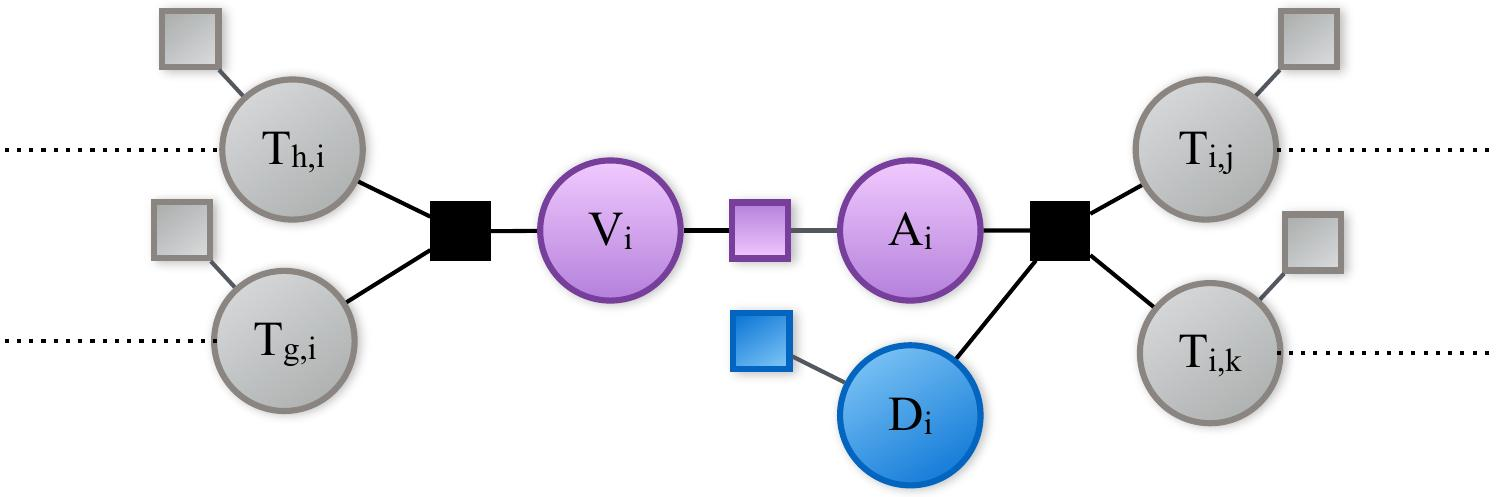
\includegraphics[width=0.8\linewidth]{model.jpeg}
\end{center}
   \caption{Factor graph for one detection with two incoming and two outgoing transition candidates. The circular nodes represent random variables, the non-black boxes describe factors that are dependent on the connected variables, and filled black boxes represent constraints. The purple detection node $i$ is seperated into a disappearance node $V_i$ and an appearance node $A_i$. The purple pairwise}
\label{fig:ctmodel}
\end{figure}

This graphical model will be reformulated into a network flow and solved as an ILP.

\subsection{ILP for Network Flow}
To solve ILPs we do LP relaxation.

Our Network flow ILP looks like this:

A LOT OF MATH

\subsection{Loosening Constraints}

On this we do cutting constraints! Because TUM something.

What we do is cut all constraints and try to solve. If it's solved, great, if not, we add constraints to nodes with flow violation. Then solve again. Repeat until we find valid solution or no new violated nodes.

\section{Experiments and Results}

Our models are: Drosophila and Rapoport (with and without mergers?)

\subsection{Solutions}

\subsection{Computation Time}


\section{Conclusion}

It works but isn't really worth it.


{\small
\bibliographystyle{ieee}
\bibliography{egbib}
}

\end{document}
